\documentclass[10pt,a4paper]{article}
\usepackage[utf8]{inputenc}
\usepackage{amsmath}
\usepackage{amsfonts}
\usepackage{amssymb}
\author{Jakob Løver, Jostein Løwer}
\title{Heisprosjekt TTK4235 \protect\\Designdokumentasjon}
\usepackage{pdfpages}
\usepackage{placeins}
\usepackage[margin=1in]{geometry}
\usepackage{tabto}




\begin{document}
\maketitle
\pagebreak
\tableofcontents
\pagebreak

\section{Introduksjon}
Målet med dette prosjektet er å designe en fungerende heis. Designet vårt skal implementeres ved hjelp av programmeringspråket C. For å oppnå dette har vi valgt å bruke V-modellen for å ferdigstille systemet. Prosjektet blir delt opp i 3 deler: en designfase, en utviklingsfase, og en godkjenningsfase.

\begin{center}
	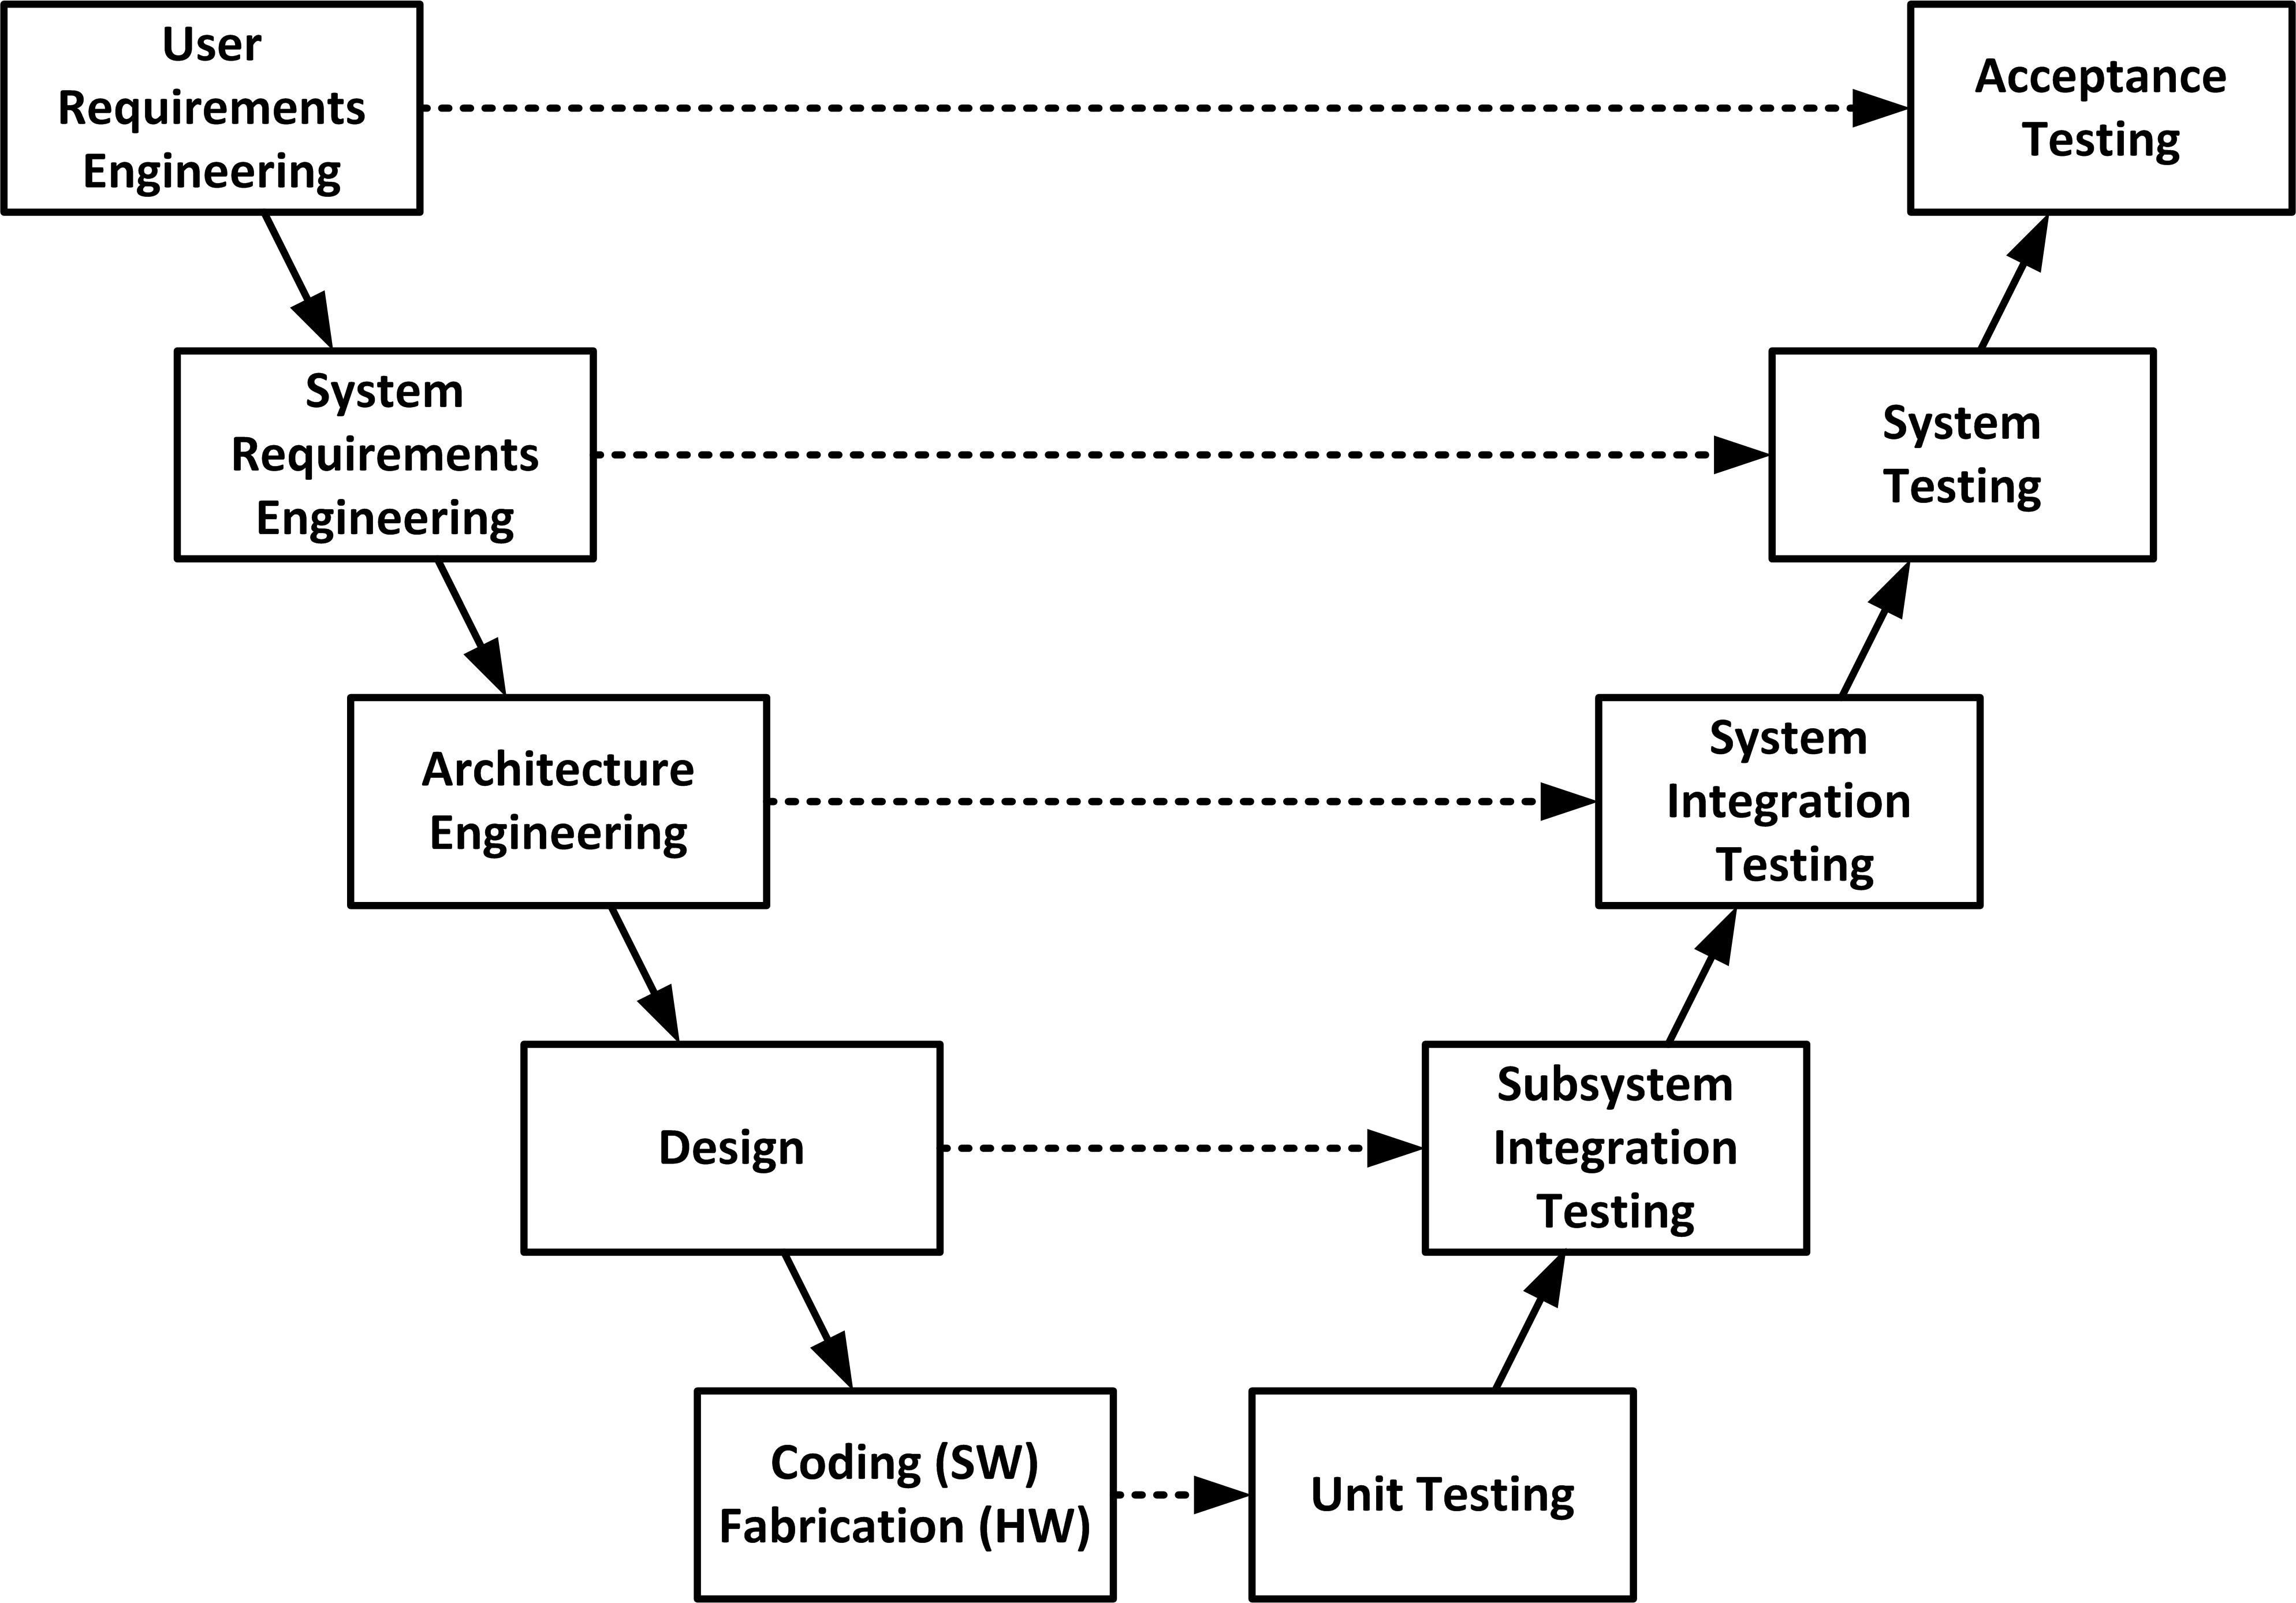
\includegraphics[scale=0.9]{v-modellen.jpg}
	\title{V-Modellen}
\end{center}



\pagebreak






\section{Use case}
\begin{center}
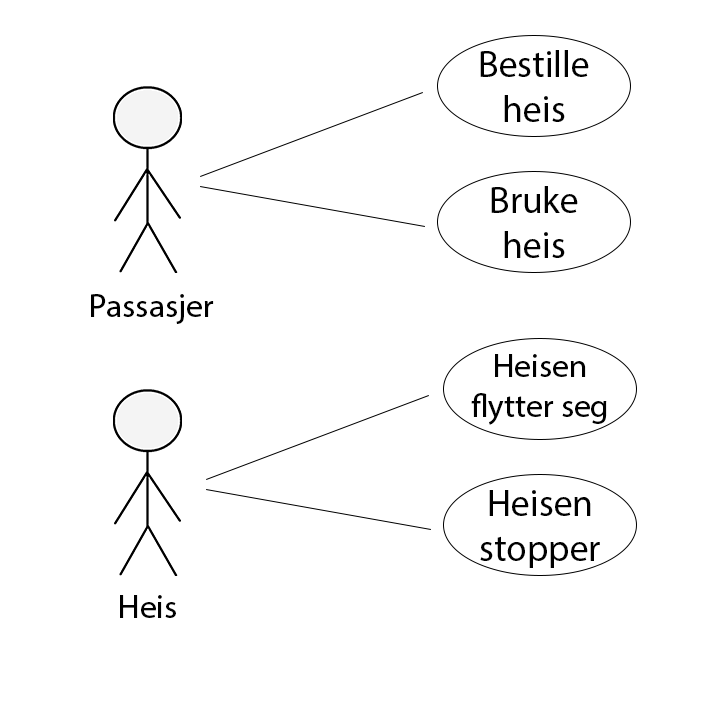
\includegraphics[scale=2]{usecase.png}
\end{center}
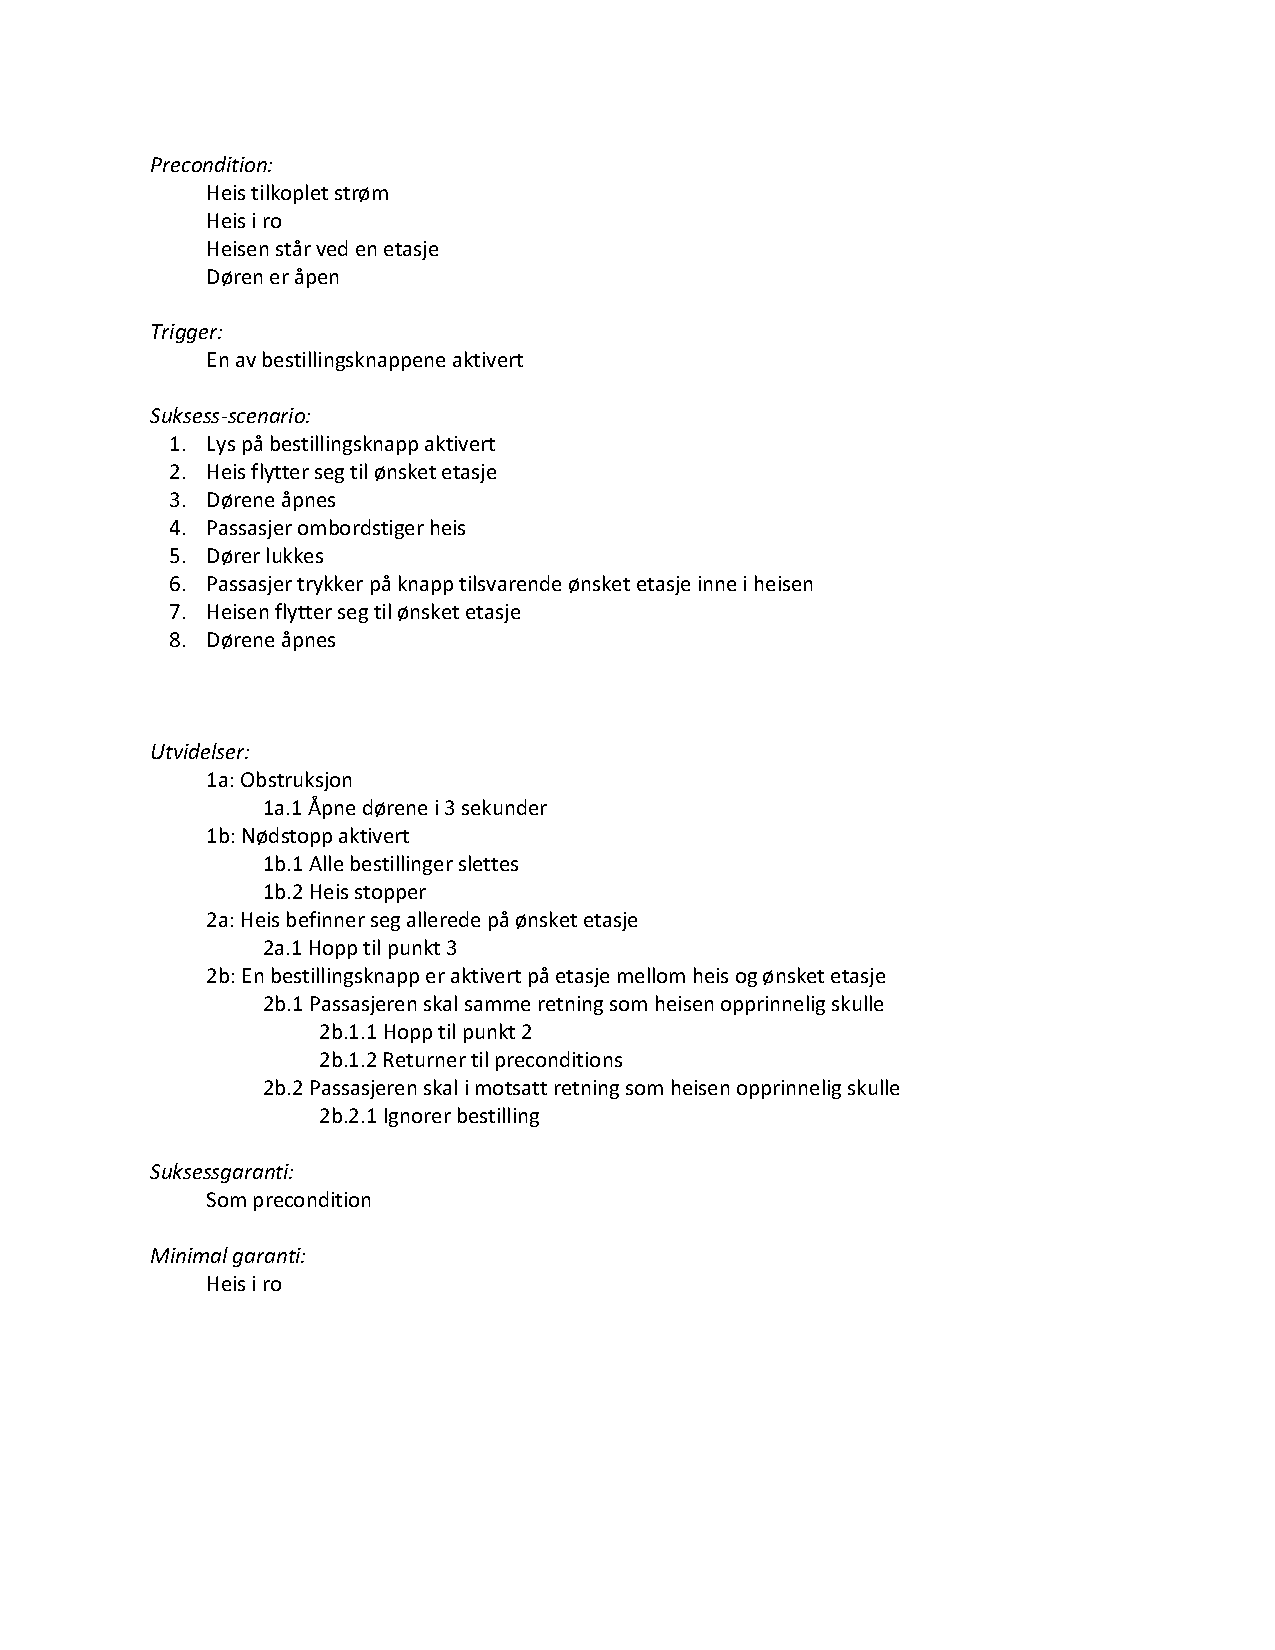
\includegraphics[scale=0.95]{usecase.pdf}






\section{Systemarkitektur}
\subsection{Klassediagram}
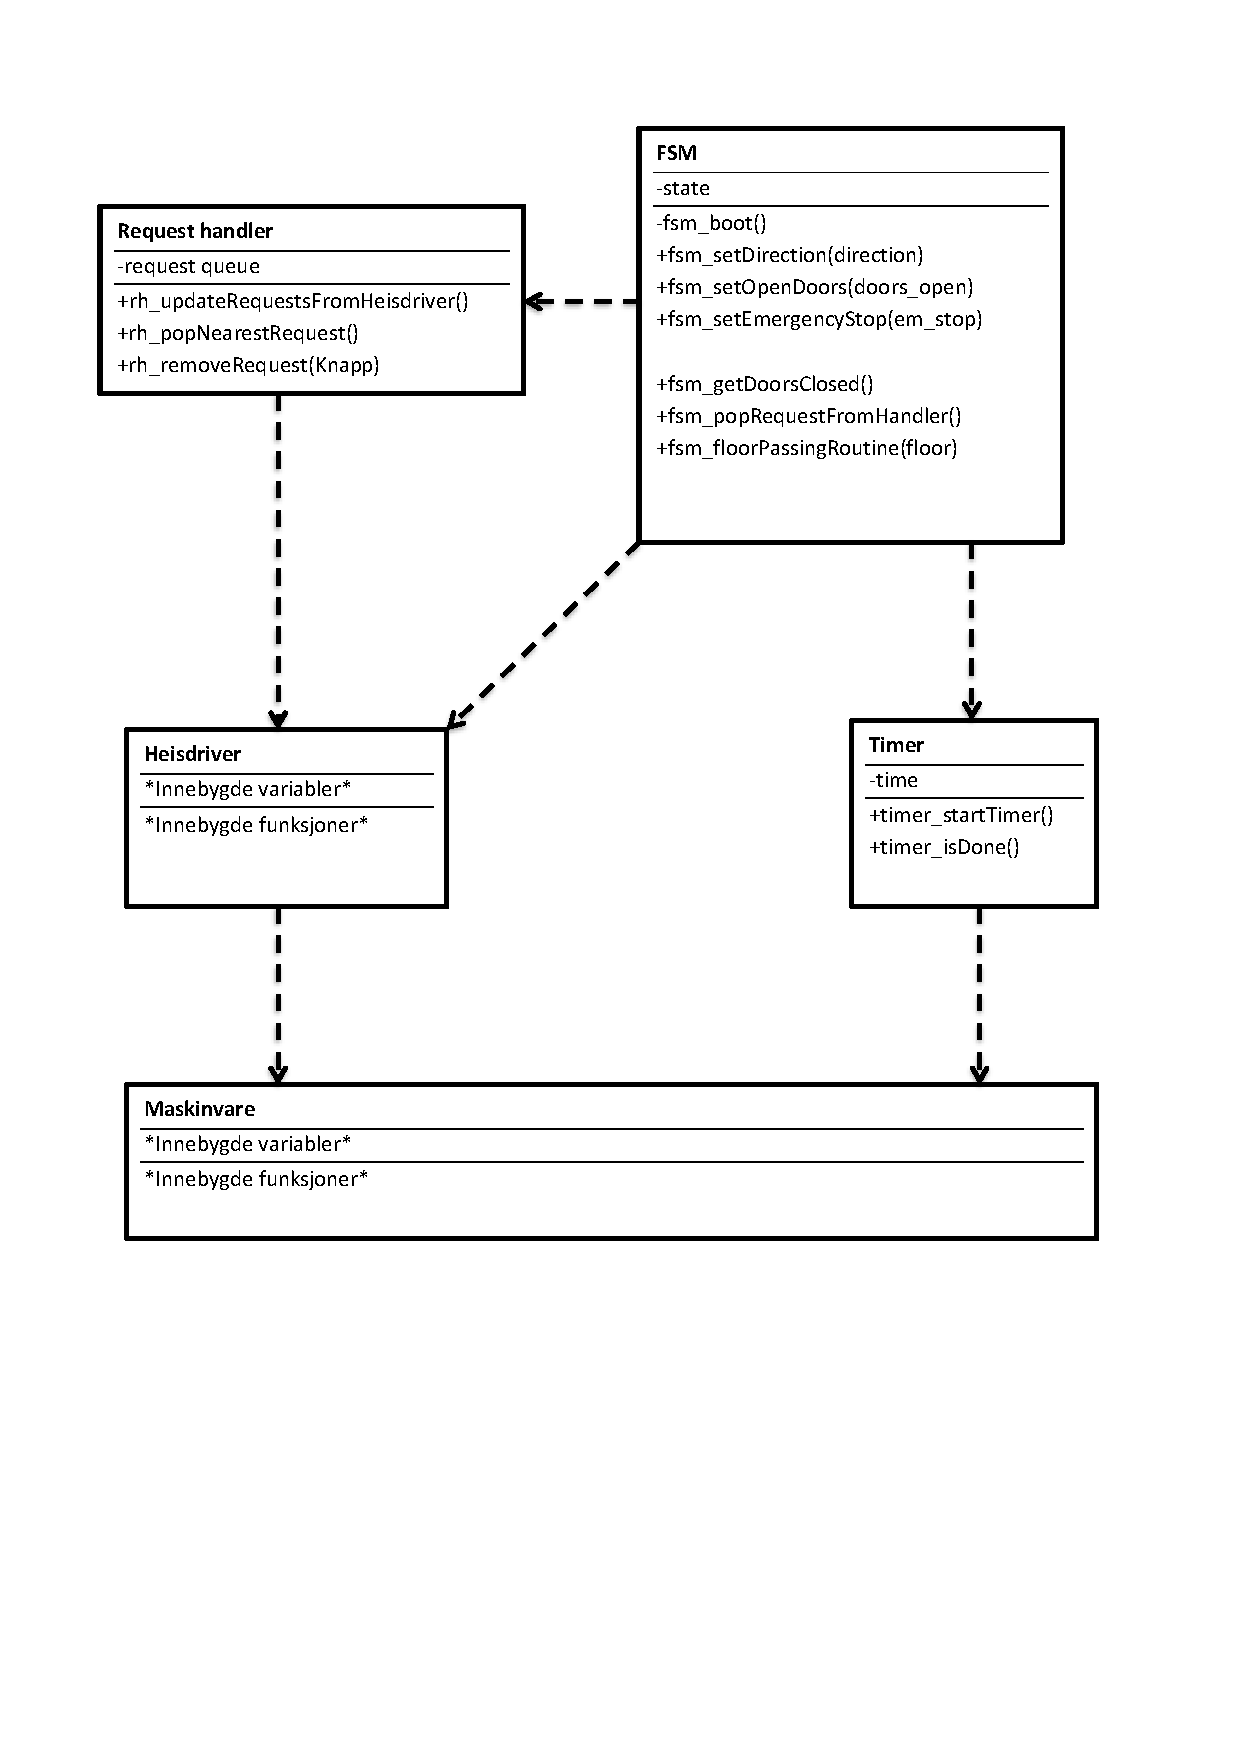
\includegraphics[scale=0.75]{Klassediagram.pdf}




\subsection{Tilstandsdiagram}
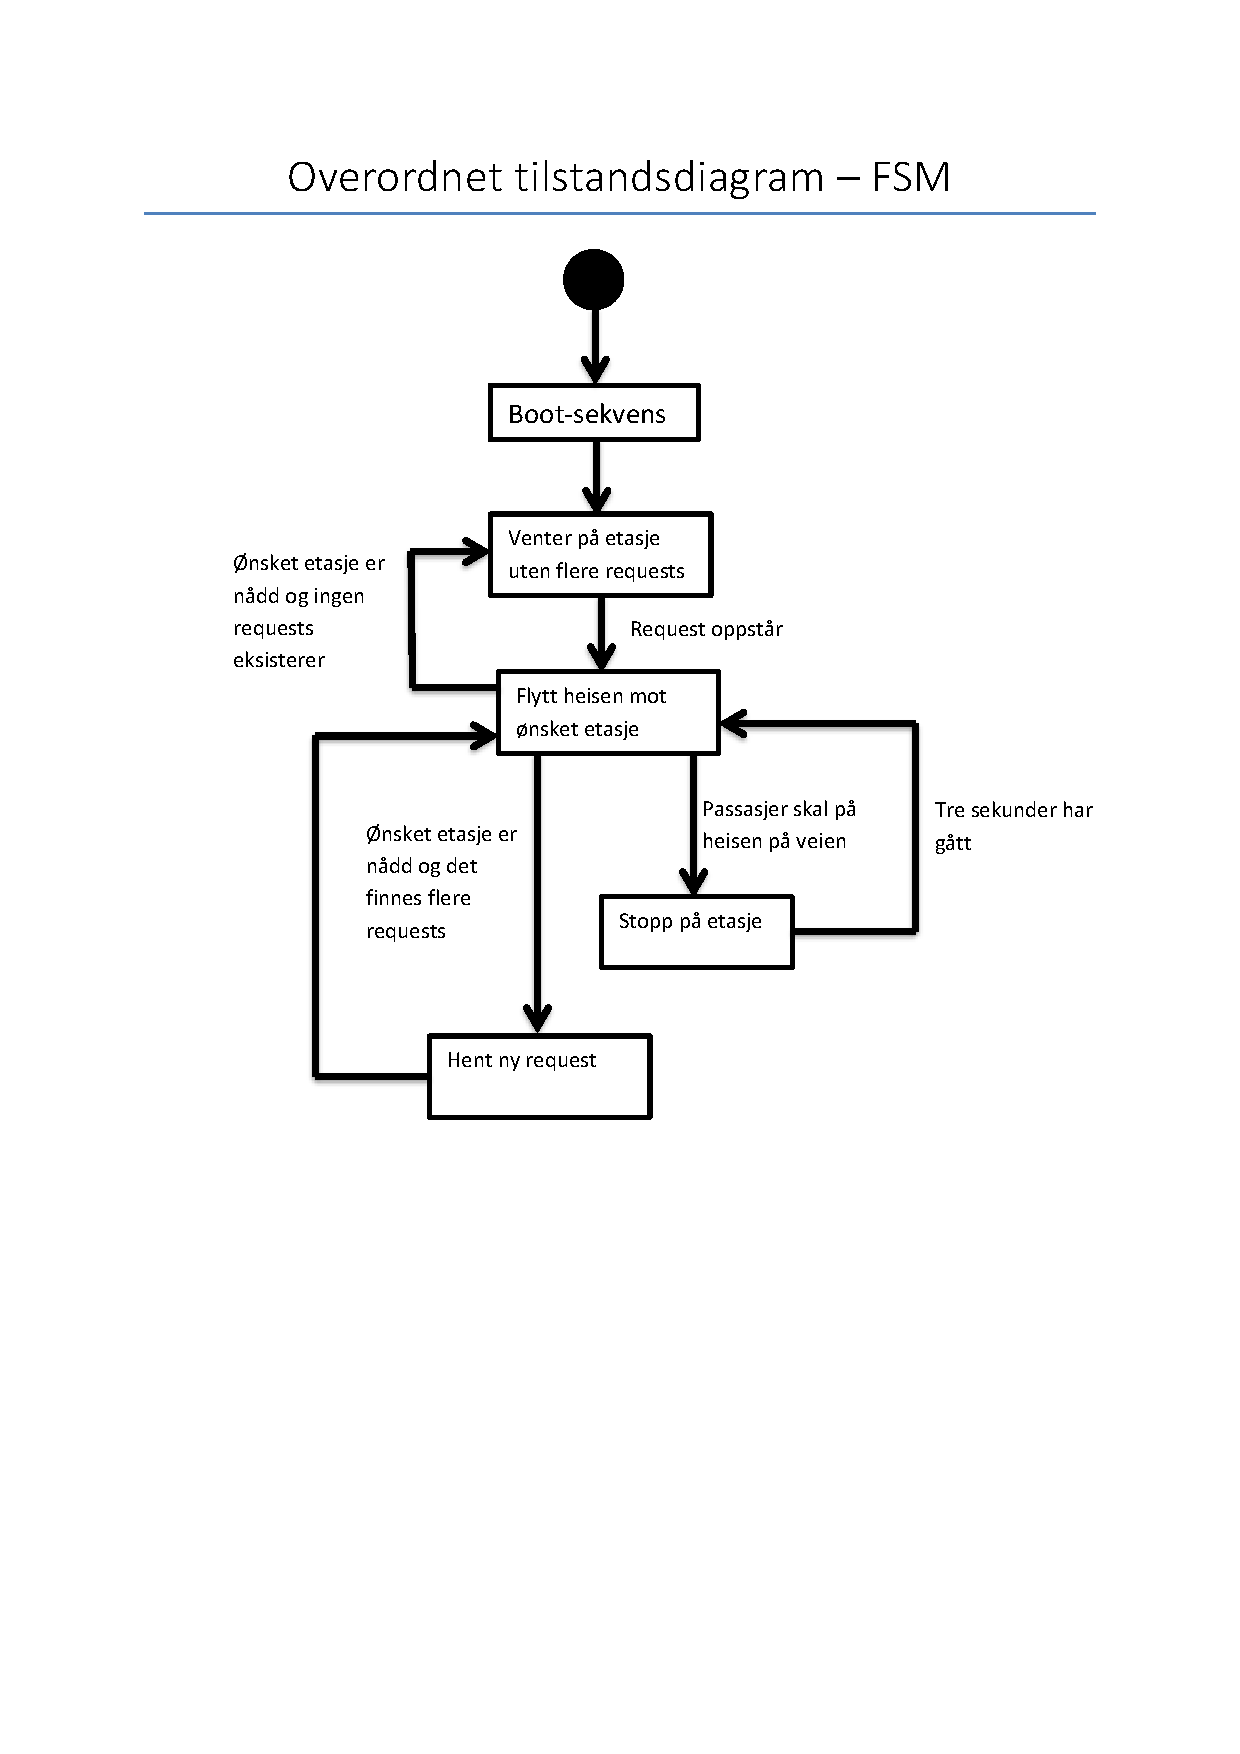
\includegraphics[scale=0.75]{overordnet_tilstandsdiagram.pdf}
\\
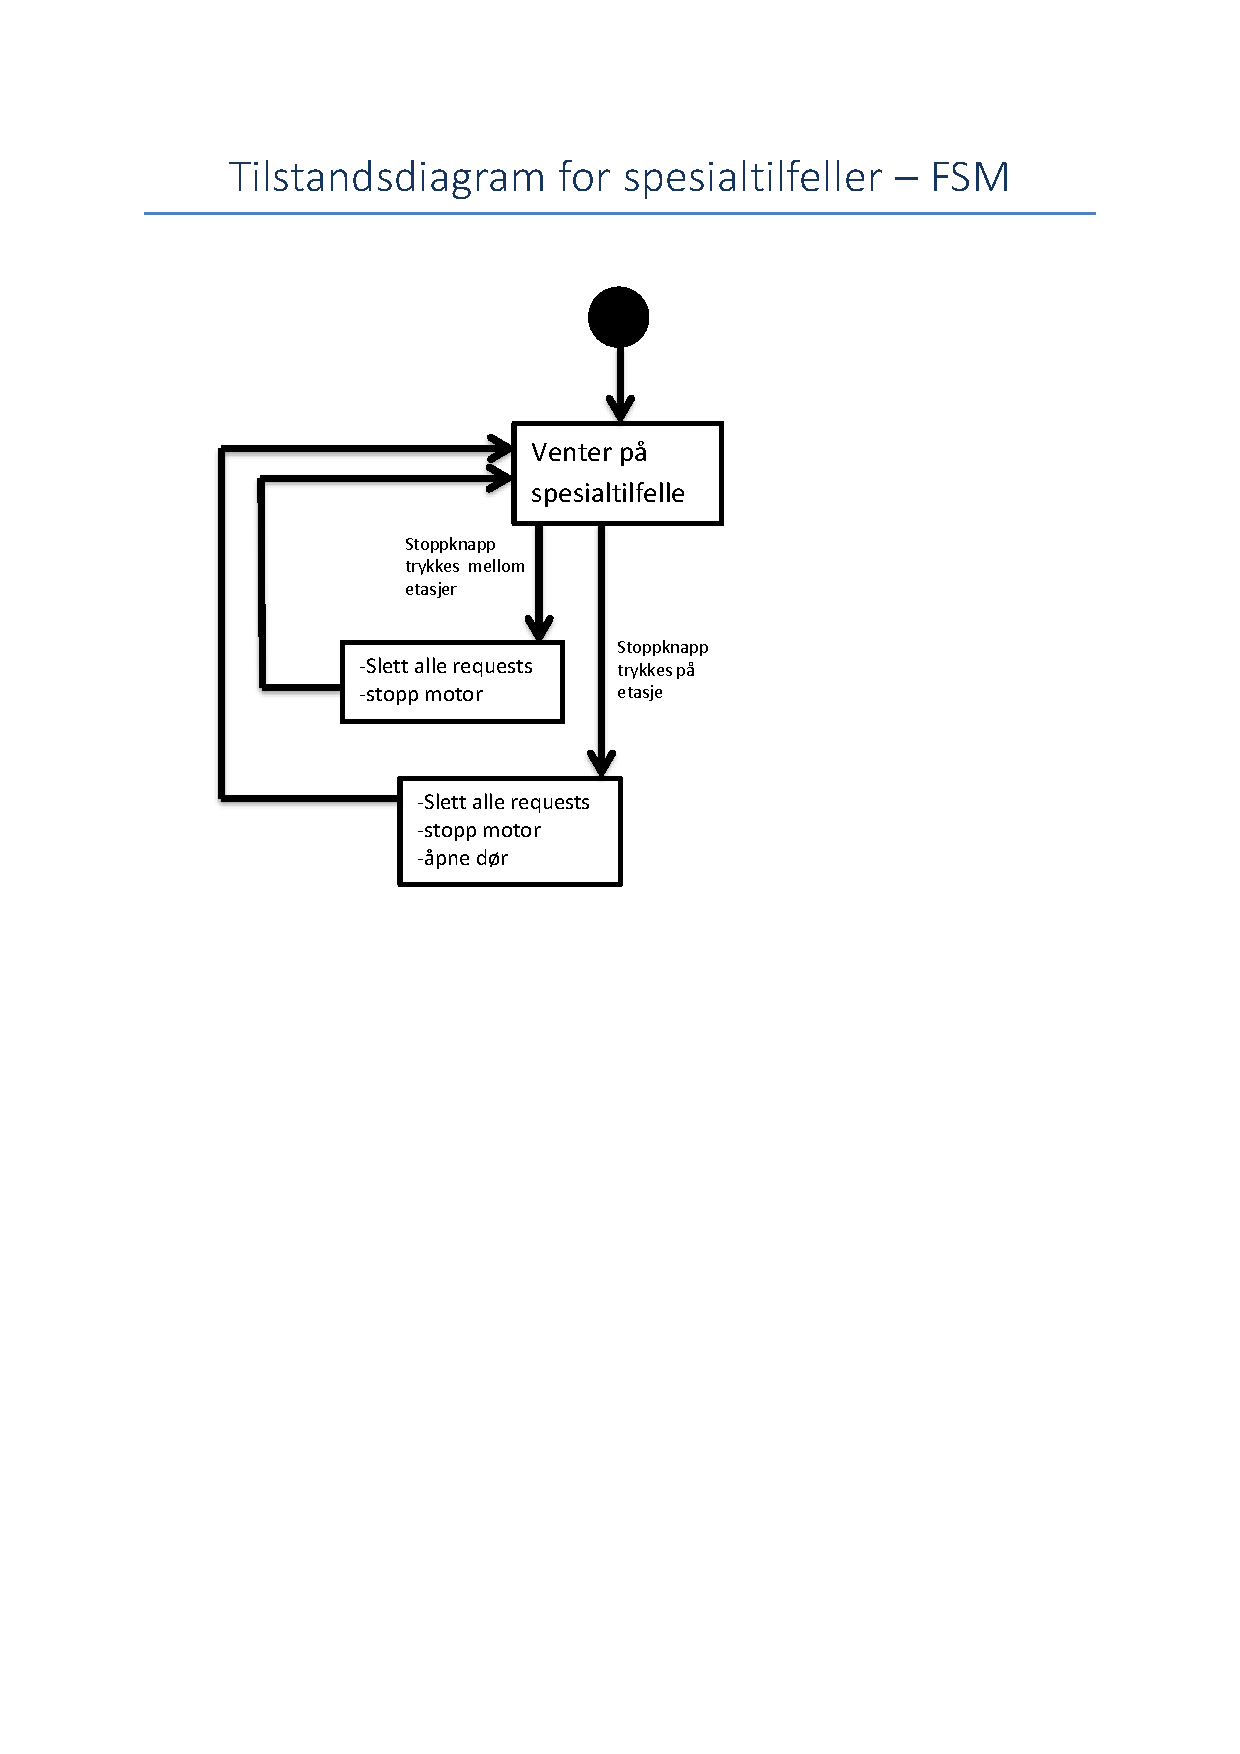
\includegraphics[scale=0.75]{spesialtilfeller_tilstandsdiagram.pdf}
\\
\pagebreak


\subsection{Sekvensdiagram}
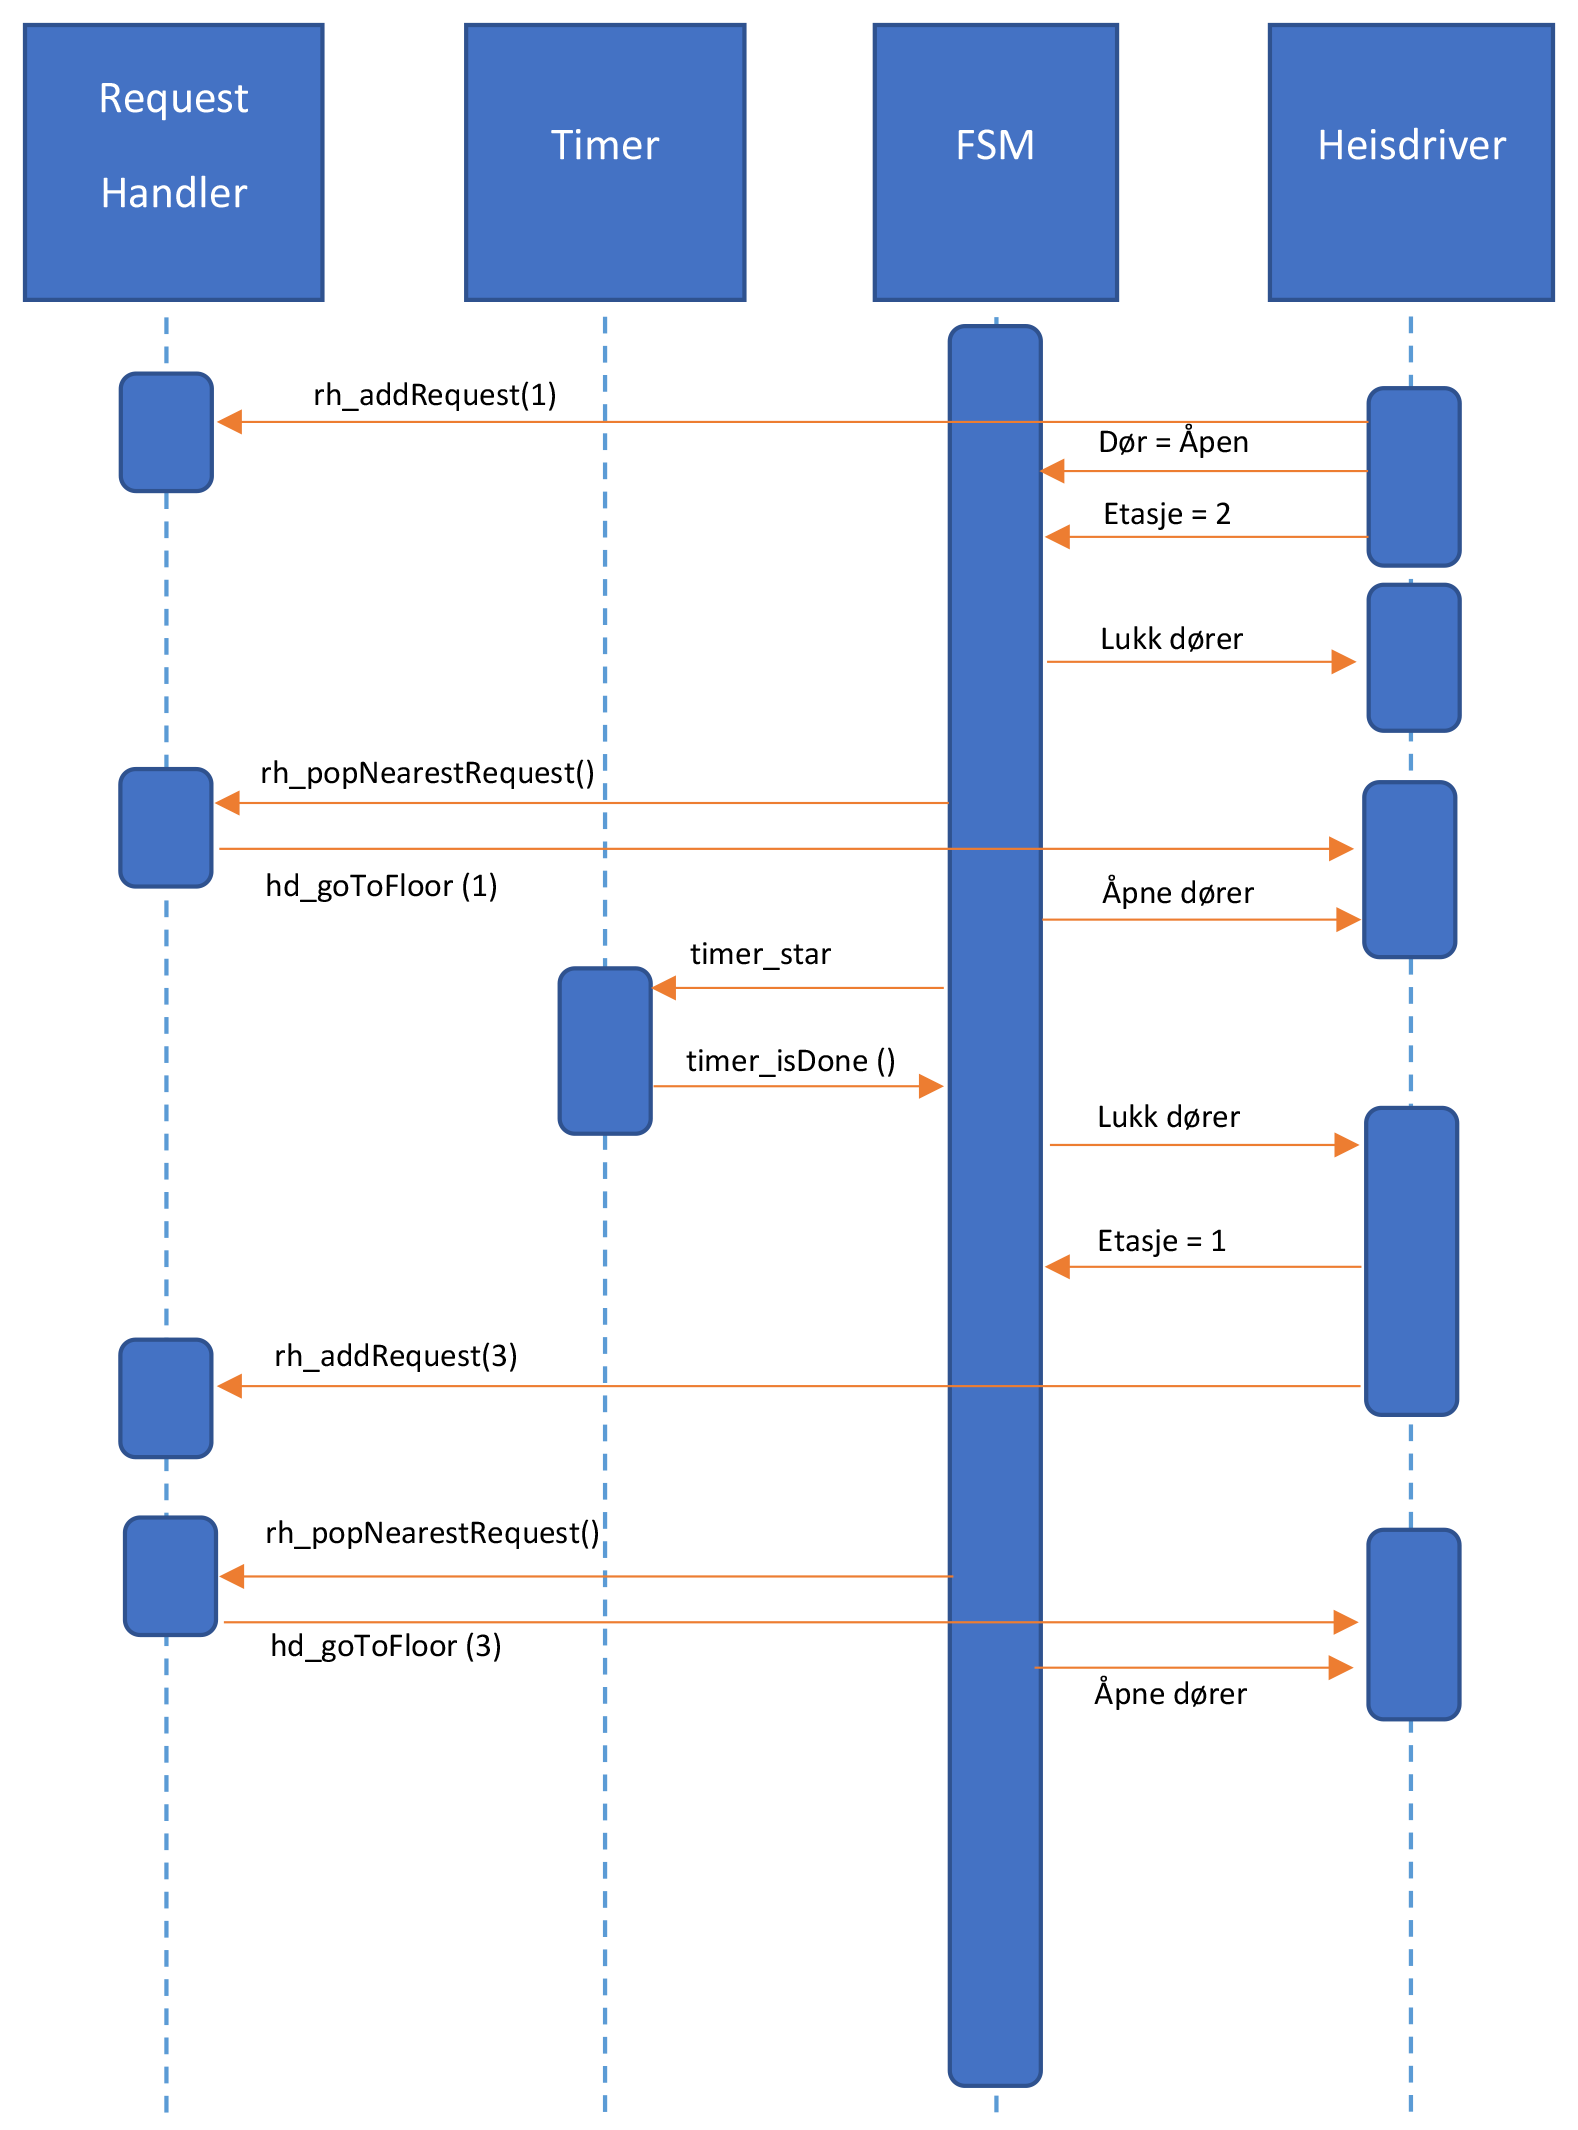
\includegraphics[scale=1]{Sekvensdiagram.png}





\end{document}